\chapter{Transistors at High Frequency}
In the BJT small-signal model of figure \ref{fig:small_signal_model3}, there are two capacitors, $C_{\pi}$ and $C_{\mu}$. These capacitors model the pn-junctions between base and emitter and base and collector, i.e. they are caused by the depletion regions. Because the emitter-base junction is forward biased and the base-collector junction is reversed biased, the depletion zone in the former junction is a lot larger than in the latter, and thus $C_{\pi} \gg C_{\mu}$.\\
We first analyze the impact of $C_{\pi}$ on the behavior of the BJT transistor at high frequencies. Next, we study the impact of $C_{\mu}$. To do this, we replace $C_{\mu}$ by a Miller capacitor $C_M$ to simplify the analysis.

\section{Giacoletto Model at High Frequencies}
In this section, we assume that $C_{\pi} \gg C_{\mu}$ and that $C_{\mu} \approx 0$. The small-signal model under these assumptions is shown in figure \ref{fig:hf_model1}. With an input current $i_b$, the base-emitter voltage is:
$$
v_{be} = \frac{r_{\pi}}{1 + j \omega r_{\pi} C_{\pi}} i_b
$$

\begin{figure}[h!]
	\centering
	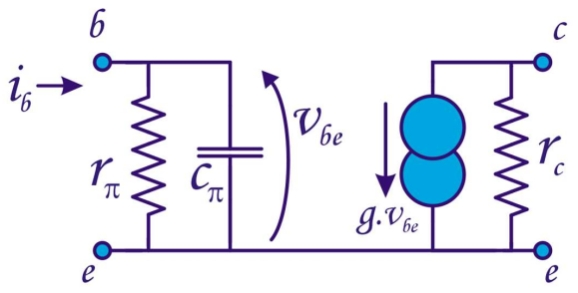
\includegraphics[width=8cm]{figures/ch03/hf_model1.jpg}
	\caption{}
	\label{fig:hf_model1}
\end{figure}
with $Z_{\pi} = \frac{r_{\pi}}{1 + j \omega r_{\pi}C_{\pi}}$ the parallel combination of $r_{\pi}$ and $C_{\pi}$. This impedance is equal to $r_{\pi}$ for low frequencies, but begins to decrease at a frequency $f_{\beta}$:
$$ 2 \pi f_{\beta} = \omega_{\beta} = \frac{1}{r_{\pi} C_{\pi}}$$
Beyond this frequency the base starts to degrade and the transistor capacity to amplify the input current decreases.\\
However, even beyond $f_{\beta}$ the transistor can still be used. He stops working when there is no current amplification, i.e. when $\frac{i_c}{i_b} = 1$, where $i_c$ is the current between collector and emitter when we short-circuit them (in the AC equivalent circuit, obviously). This short-circuit current gain $A_{i, sc}$ is the ratio of the current generated by the dependent current source with respect to the input current:
$$
A_{i, sc} = \frac{i_c}{i_b} = g \; v_{be} = g  \frac{r_{\pi}}{1 + j \omega r_{\pi}C_{\pi}}
$$
We compute the pulsation $\omega_T$ when $| A_{i, sc} | = 1$:
\begin{align*}
	\Bigg| g  \frac{r_{\pi}}{1 + j \omega r_{\pi}C_{\pi}} \Bigg| &= 1 \\
		= \frac{g r_{\pi}}{\sqrt{1 + \frac{\omega^2}{\omega_{\beta}^2}}} 
		&= \frac{\beta}{\sqrt{1 + \frac{\omega^2}{\omega_{\beta}^2}}}
\end{align*}
because $g \; r_{\pi} = \frac{I_{CQ}}{v_{th}} \frac{v_{th}}{I_{BQ}} = \frac{I_{CQ}}{I_{BQ}} = \beta$. Consequently:
\begin{align*}
	\omega_{\beta}^2 \beta^2 &= \omega_{\beta}^2 + \omega^2 \\
	\Rightarrow \omega &= \omega_{\beta} \sqrt{\beta^2 - 1} \approx  \omega_{\beta} \beta
\end{align*}
This pulsation $\omega_T = \beta \; \omega_{\beta}$ is the pulsation beyond which the BJT no longer amplifies the current and thus becomes useless.

\section{The Miller Capacitor}
\label{sec:miller_cap}
In this section, we will also take $C_\mu$ into account. We study the common-emitter amplifier from figure \ref{fig:amplifier7} when the input signal $v_i$ has high-frequency components. We assume that both $C_B$ and $C_E$ are short circuits, i.e. we are in the correct working domain (the right part of the Bode curve in figure \ref{fig:amplifier6}). With both $C_{\pi}$ and $C_{\mu}$ present, and an output impedance $R_S$ of the signal source, we obtain the AC circuit from figure \ref{fig:hf_model2}.

\begin{figure}[h!]
	\centering
	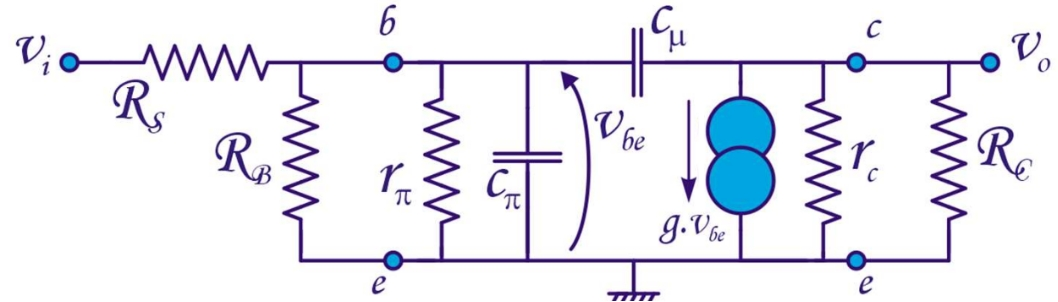
\includegraphics[width=12cm]{figures/ch03/hf_model2.jpg}
	\caption{}
	\label{fig:hf_model2}
\end{figure}
The difficulty in this circuit is the presence of $C_{\mu}$: this capacitor couples the base to the collector, making the analysis hard. To proceed, we want to remove $C_{\mu}$ and replace it by something else, like an element in parallel with $C_{\pi}$. This is where the Miller capacitor comes in.\\
The key insight is that we can replace the series capacitor $C$ in figure \ref{fig:milcap1}, which induces a current $i = j \omega C (v_2 - v_1)$, by the two loops in figure \ref{fig:milcap2}. From an electrical point of view, these circuits are identical because the currents and voltages at the in- and output terminals are identical.

\begin{minipage}{.5\textwidth}
	\centering
	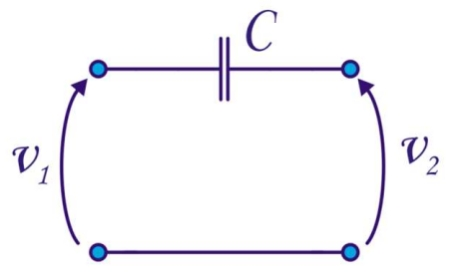
\includegraphics[width=6cm]{figures/ch03/milcap1.jpg}
	\captionof{figure}{}
	\label{fig:milcap1}
\end{minipage}%
\begin{minipage}{.5\textwidth}
	\centering
	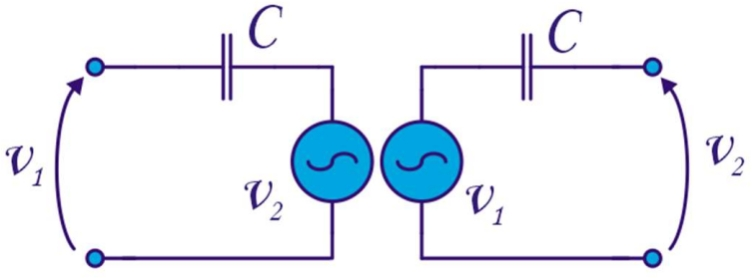
\includegraphics[width=7cm]{figures/ch03/milcap2.jpg}
	\captionof{figure}{}
	\label{fig:milcap2}
\end{minipage}

In the right loop, we replace the voltage source with its Norton equivalent $i_N = j \omega C v_1$, as in figure \ref{fig:milcap4}.

\begin{figure}[h!]
	\centering
	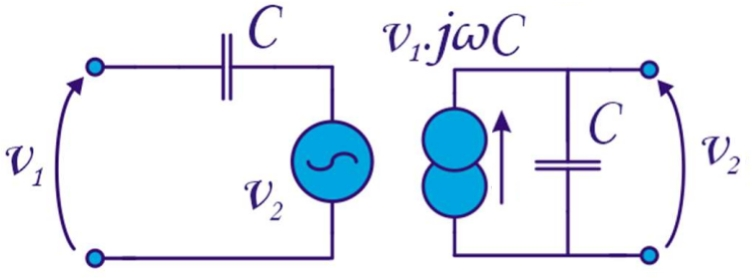
\includegraphics[width=10cm]{figures/ch03/milcap4.jpg}
	\caption{}
	\label{fig:milcap4}
\end{figure}

If we replace $C_{\mu}$ in this way in the AC-circuit of figure \ref{fig:hf_model2}, we obtain the circuit in figure \ref{fig:milcap5}. Note that $Z_\pi$ is $r_\pi || C_\pi || R_B$ and $R_{eq} = r_c || R_C$. In this circuit, we will now:
\begin{itemize}
	\item Neglect current source $v_{be} j \omega C_{\mu}$ when it is dominated by $ g\;  v_{be}$. This is valid when:
	\begin{align*}
		v_{be} j \omega C_{\mu} &\ll g\;  v_{be}\\
		| j \omega C_{\mu}| &\ll |g| \\
		\rightarrow \omega &\ll \omega_1 = \frac{g}{C_{\mu}}
	\end{align*}
	This is the first criterion: $\omega \ll  \frac{g}{C_{\mu}}$
	\item Neglect $C_{\mu}$ in the output loop because its impedance is lot larger then $R_{eq}$. This is valid if:
	\begin{align*}
		\frac{1}{j \omega C_{\mu}} &\gg R_{eq} = r_c || R_C\\
		\rightarrow \omega &\ll \omega_2 = \frac{1}{R_{eq}C_{\mu}}
	\end{align*}
	This is the second criterion: $\omega \ll  \frac{1}{R_{eq}C_{\mu}} $
\end{itemize}
\begin{figure}[h!]
	\centering
	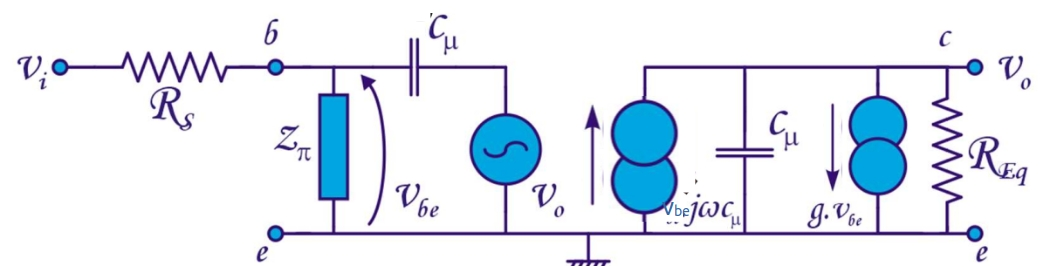
\includegraphics[width=12cm]{figures/ch03/milcap5.jpg}
	\caption{}
	\label{fig:milcap5}
\end{figure}
Note that in a typical scenario, e.g. with $I_{CQ} = 1$ mA and $R_C = 1$ k$\Omega$, $g \gg G_C$ and $g \gg g_c$ (this is always valid) and thus mostly $g \gg G_c + g_c = \frac{1}{R_{eq}}$. So if the second criterion is valid, the first will be valid as well. In general, the Miller conditions are satisfied.\\
After neglecting $j \omega \; C_\mu  \;  v_{be}$ and $C_\mu$, the small-signal circuit becomes the one in figure \ref{fig:milcap6}. In this circuit, we know that $v_o = -g \; R_{eq} \; v_{be}$. Hence, the current though $C_\mu$ in the left loop is equal to:
\begin{align*}
	i_{C_\mu} &= j \omega C_\mu (v_{be} - v_o) \\
			  &= j \omega C_\mu (1 + g \; R_{eq}) \; v_{be}
\end{align*}
So we can replace $C_\mu$ and the source that provides $v_o$ by a single capacitor with capacitance $C_\mu (1 + g \; R_{eq})$. This is the Miller capacitor:
\begin{equation}
	C_M = C_\mu (1 + g  R_{eq})
	\label{eq:miller_cap}
\end{equation} 
as in figure \ref{fig:milcap7}. 

\begin{minipage}{.5\textwidth}
	\centering
	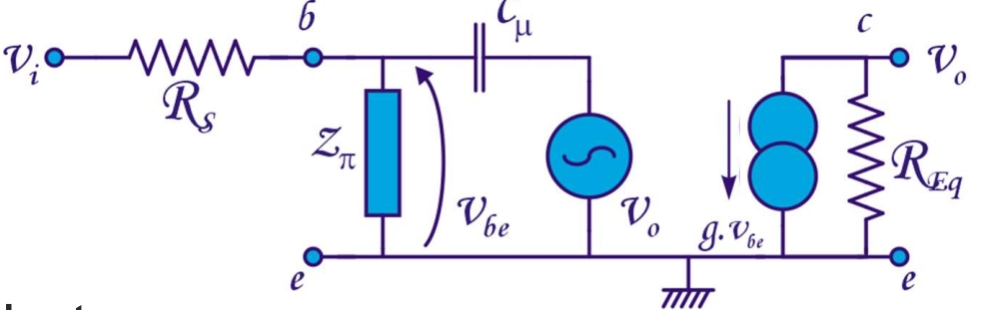
\includegraphics[width=8cm]{figures/ch03/milcap6.jpg}
	\captionof{figure}{}
	\label{fig:milcap6}
\end{minipage}%
\begin{minipage}{.5\textwidth}
	\centering
	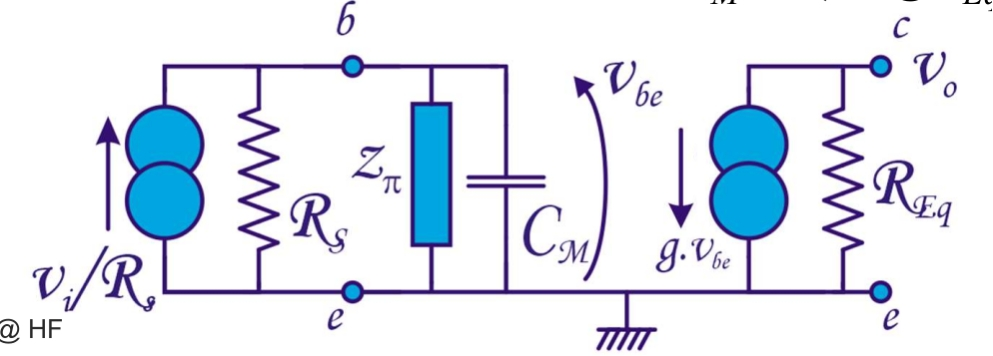
\includegraphics[width=7cm]{figures/ch03/milcap7.jpg}
	\captionof{figure}{}
	\label{fig:milcap7}
\end{minipage}
We can in the left loop of figure \ref{fig:milcap7} group al impedance in a single $Z_{eq} = \frac{R}{1 + j \omega R(C_\pi + C_M)}$ with $R = r_\pi || R_B || R_S$ the parallel combination of all resistors in the input part of the circuit, and $C_\pi + C_M$ the parallel combination of $C_\pi$ and $C_M$. The base-emitter voltage is then equal to:
$$
v_{be} = \frac{1}{R_S} \frac{R}{1 + j \omega R(C_\pi + C_M)} v_i
$$
and the voltage gain is:
$$
A_v = \frac{v_o}{v_i} = - g R_{eq} \frac{v_{be}}{v_i} = - g R_{eq} \frac{1}{R_S} \frac{R}{1 + j \omega R(C_\pi + C_M)}
$$
When $R_S$ is small, $R \approx R_S$ and:
\begin{equation}
	A_v \approx - g  \frac{R_{eq}}{1 + j \omega R(C_\pi + C_M)}
	\label{eq:miller_gain}
\end{equation}


\section{Miller's Theorem}
\label{sec:miller_theorem}
Equation \ref{eq:miller_cap} is an instance of Miller's theorem, which aims to replace a floating impedance with two grounded impedances as we did in figure \ref{fig:milcap1}. For the derivation, refer to figure \ref{fig:miller}.

\begin{figure}[h!]
	\centering
	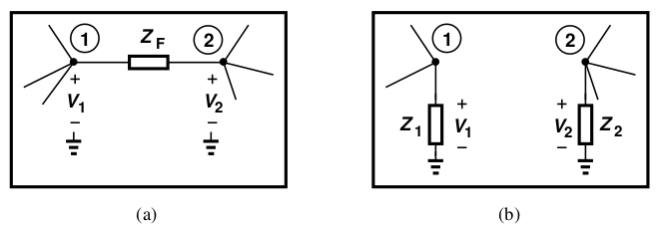
\includegraphics[width=12cm]{figures/ch03/miller.jpg}
	\caption{}
	\label{fig:miller}
\end{figure}
We wish to transform $Z_F$ to two grounded impedances as depicted in figure \ref{fig:miller}(b), while ensuring all of the currents and voltages in the circuit remain unchanged. This means:
\begin{align*}
	\frac{V_2 - V_1}{Z_F} &= \frac{V_1}{Z_1} \\
	\frac{V_1 - V_2}{Z_F}  &= -\frac{V_2}{Z_2}
\end{align*}
If we denote the voltage gain from node $1$ to node $2$ as $A_v = \frac{V_2}{V_1}$, we find:
\begin{align*}
	Z_1 &= \frac{V_1}{V_2 - V_1} Z_F\\
		&= \frac{1}{1-A_v} Z_F
\end{align*}
for $Z_1$ and 
\begin{align*}
	Z_2 &= \frac{V_2}{V_1 - V_2} Z_F\\
	&= \frac{1}{1-A_v^{-1}} Z_F
\end{align*}
for $Z_2$.
\section{Conclusion}
At high frequencies, we must take the parasitic capacitances of the transistor into account. For floating capacitances like $C_\mu$, we use Miller's theorem and replace it by $C_M$. Note that we can only do this if the Miller conditions are satisfied:
\begin{enumerate}
	\item $\omega \ll \frac{g}{C_\mu}$
	\item $\omega \ll \frac{1}{R_{eq} C_\mu}$
\end{enumerate}
 From equation \ref{eq:miller_gain}, we see that there is a cut-off frequency for the gain:
$$
\omega_H = \frac{1}{c_\pi + C_M}
$$
Above this frequency, the gain $A_v$ of the common-emitter amplifier begins to decrease, and we can extend figure \ref{fig:amplifier6} to include this cut-off frequency, as in figure \ref{fig:milcap8}. We also know that $\omega_H < \frac{1}{r_\pi C_\pi} = \omega_\beta$. This means that performance degradation is initially due to a direct signal path from base to collector through $C_\mu$, and that base degradation happens later (i.e. at higher frequencies).

\begin{figure}[h!]
	\centering
	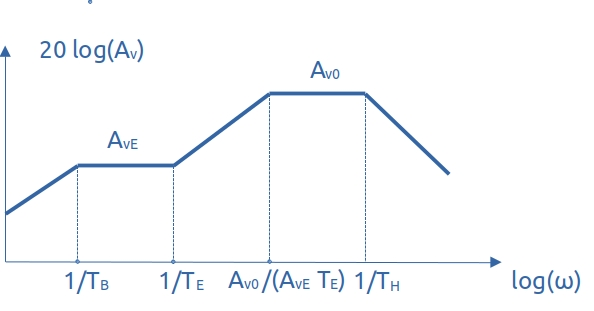
\includegraphics[width=12cm]{figures/ch03/milcap8.jpg}
	\caption{}
	\label{fig:milcap8}
\end{figure}